\chapter{Numerical Experiments}
\label{chapter:NumericalExperiments}

\section{Cantilever Beam}
\subsection{Problem Description}
% Youns modulus 1,000,000
% poisson = 0.3
% density = 0.001
% units?

% newton load steps
% setup of beam pictures
% discretization strategy (maybe table of values?)
% tartaros setup variables
% \begin{figure}[hbt]
%     \centering
% \begin{circuitikz}
%     %wall
%     \fill[pattern=north east lines] (0,.5) rectangle (0.25,4);
%     \draw (0.25,.5) -- (0.25,4);
%     % beam
%     \draw[fill=gray!40] (0.25,2) rectangle (6,2.5);
%     % length of beam
%     \draw[<->|] (0.25,1.8) -- (6,1.8) node[midway,below] {$L$};
%     % force
%     \draw[->] (6,4) -- (6,2.5) node[midway,left] {$F$};
%     \draw[dashed] (6,2.5) -- (9,2.5);
%     \draw[dashed] (6,2) -- (9,2);
%     \draw[fill=gray!40] (9,2) rectangle (10,2.5);
%     \draw[] (9,1.8) -- (10,1.8) node[midway,below] {$w$};
%     \draw[|<->|] (10.2,2) -- (10.2,2.5) node[midway,right] {$h$};
% \end{circuitikz}
% \end{figure}

To compare the performance of a Krylov solver preconditioned with SA-AMG with that of a direct solver, a scaling study was performed on two different 3 dimensional cantilever beams of varying height $h$. The factor $r$, chosen to be 10 and 100, determined the ratio of length-to-height. The beam material was a Neo-Hooke material with a Young's modulus of $E = 10\ \text{MPa}$ and a Poisson's ratio of $\nu = 0.3$. The beam shown in Figure~\ref{fig:beam} is fixed with Dirichlet boundary conditions on one end and has a Neumann load on the other end. The beams were discretized with 8 node hexahedral elements, and for two studies the amount of elements was varied in increments of $10^4$ for one study and $10^6$ for the other. For the discretization elements, the condition was imposed that the element aspect ratio remain as close to 1 as possible, such that the elements were cube-shaped.

% machine setup

\begin{figure}[h]
    \centering
    \begin{tikzpicture}
    
    % \draw[->] (0,0,0)-- node[pos=.7,below] {x} ++(6,0,0);
    % \draw[->] (0,0,0)--++(0,3,0) node[pos=.75, left=7mm,rotate=90]{y};
    % \draw[->] (0,0,0)--++(0,0,4) node[midway, sloped, above] {z};
    % \fill (10,0.1,1) circle(3pt);
    \draw[pattern=north west lines] (0,1,1.5)--(0,-0.5,1.5)--(0,-0.5,-1)--(0,1,-1)--cycle;

    \draw[fill=gray!40] (10,0.5,1)--(10,0.5,0)--(0,0.5,0)--(0,0.5,1)--cycle node[midway, above, yshift=0.82 cm] {$E = 1$ MPa\ \ \ $\nu = 0.3$}; %top
    \draw[fill=gray!40] (10,0.5,1)--(10,0,1)--(10,0,0)--(10,0.5,0); %right
    \draw[fill=gray!40] (10,0,1)--(0,0,1)--(0,0.5,1)--(10,0.5,1) -- cycle; %front

    \draw[dim] (0,-0.75,1.2) -- (10, -0.75, 1.2) node[midway, below] {$L = 10$ m};
    \draw (0, -0.5, 1) -- (0, -0.9, 1.2);
    \draw (10, -0.5, 1) -- (10, -0.9, 1.2);
    \draw[dim] (10,-0.5,0.5) -- (10, -0.5, -0.5) node[midway, below, xshift=0.7cm] {$w = 1$ m};
    \draw (10, -0.4, 0.6) -- (10, -0.6, 0.4);
    \draw (10, -0.4, -0.4) -- (10, -0.6, -0.6);
    \draw[dim] (10.5, 0, 0) -- (10.5, 0.5, 0) node[midway, right] {$h = L/r$};
    \draw (10.4, 0, 0) -- (10.6, 0, 0);
    \draw (10.4, 0.5, 0) -- (10.6, 0.5, 0);
    \draw (10.0, 0.5, 0) -- ++(0, 0, 1.0) node[midway, above, yshift=0.4 cm] {$F = \frac{1}{(r/10)^3}$ N/m};
    \foreach \z in {0,0.25,...,1} {
        \draw[-latex] (10.0,0.5,\z) -- ++(0,-0.5,0);
    }

    % \fill[pattern=north east lines] (0,.5,0) rectangle (0.5,0.25,1);

\end{tikzpicture}
\caption{3 dimensional cantilever beam}
\label{fig:beam}
\end{figure}

% describe the solver setup
The solver consists of a nonlinear Newton solver performing a time integration scheme, although the problem being considered is non-transient. At each Newton iteration, a linear system of equations has to be solved. The load $F$ starting at 0 is increased by a constant amount each time step so that it reaches the desired load value at the final time step. This is done to give the Newton statics solver better convergence properties, since the incrementally applied load results in the solution being within the method's radius of convergence. For this experiment, 10 load steps were used, and the statics solver was considered converged if the residuals for the Newton iterations were below $10^{-5}$.

Within each Newton iteration, the system of equations is solved with a GMRES method that is preconditioned with an SA-AMG solver. The GMRES convergence criterion of $\norm{r_k}_2/\norm{r_0}_2 < 10^{-6}$ was used, with a maximum number of iterations of 1000. The particular implementation was a restarted GMRES which would restart after the Krylov subspace reached a chosen size of 100.

\begin{table}[ht]
    \centering
    \begin{tabular}{|l|l|} 
    \hline
    Setting Name & Value \\
    \hline
    Cycle Type                          & V                     \\
    Max Levels                          & 7                     \\
    Muelu Reuse Strategy                & Nothing               \\
    PDE Equations                       & 3                     \\
    \hline
    Aggregation: Type                    & Uncoupled             \\
    Aggregation: Damping Factor          & 1.33                  \\
    Aggregation: Nodes Per Aggregate    & 27                    \\
    \hline
    Smoother: Sweeps                     & 1                     \\
    Smoother: Damping Factor             & 1                     \\
    Smoother: Pre- or Post-Smoothing     & Both                  \\
    Smoother: Type                       & Chebyshev             \\
    Chebyshev Degree (Fine to Coarse)       & 12, 6, 6, 6, 6, 6, 1  \\
    Eigen-Analysis: Type                 & CG                    \\
    Eigen-Analysis: Iterations           & 10                    \\
    \hline
    Coarse-Level: Solver                 & Amesos-UMFPACK        \\
    Coarse-Level: Max Size               & 20000                 \\
    Coarse-Level: Pre- or Post-Smoothing & Pre                   \\
    Coarse-Level: Sweeps                 & 1                     \\
    Coarse-Level: Split Communicator     & False                 \\ 
    \hline
    Repartitioning                      & Enabled               \\
    Repartitioner                       & ParMETIS              \\
    Repartitioning: Max-Min Ratio       & 1.2                   \\
    Repartitioning: Min per Proc        & 1000                  \\
    \hline
    \end{tabular}
    \caption{MueLu Settings used for various numerical experiments}
    \label{table:muelu}
\end{table}

The SA-AMG preconditioner was set up with the MueLu settings from Table~\ref{table:muelu}. The maximum amount of level was limited to 7, and a coarse level size of 20000 DOFs was used in order to limit the amount of coarsening.

The Chebyshev polynomial smoother was used, since the computational kernel involves a matrix-vector product which works well for SPD matrices. This smoother requires estimates of minimum and maximum eigenvalues of $A$, and recursively forms Chebyshev polynomials of increasing degree which are used to form the residual. The full method is detailed in Gutknecht et al.~\cite{Gutknecht2002}. The degree of the polynomial is reduced at coarser levels to reduce the amount of computation. At the coarsest level, the problem is solved with the UMFPACK solver from the Amesos library, which is a direct sparse LU factorization method~\cite{Davis2004}.

The uncoupled aggregation strategy is used, which avoids aggregating nodes which are assigned to different processors. This aggregation method has the advantage of reducing communication between processors during aggregation as well as prolongator smoothing, but can result in some aggregates near processor boundaries being too small. Since aggregates cannot cross processor boundaries, the coarse level problem might have too many nonzeroes per row. Additionally, some processors could have more work than others on the coarse level, which results in other processors having to wait (\cite{Tuminaro2000}, ~\cite{Hu2014}). The number of nodes per aggregate was chosen to be 27 for the 3D problem, since aggregates having a diameter of less than three can lead to high iteration costs~\cite{Tuminaro2000}.

With the uncoupled aggregation process, rebalancing the problem among the processors is necessary. This is implemented with the ParMETIS library, and reduces the number of processors on coarse levels such that a minimum amount of DOFs of 1000 per processor is achieved. The problem is also rebalanced if any processor has more than 1.2 times the amount of nonzeroes as another processor.

\subsection{Results}
The simulations were run with up to 40 total cores on 4 Intel Xeon Silver 4114 processors. The first study had a target amount of $10^4$ elements per MPI rank at the finest level. This corresponds to approximately 30,000 DOFs per core. The combined wall clock times spent in both the GMRES solver and AMG preconditioner as well as the number of GMRES iterations are shown in Figure~\ref{fig:weak_scaling}. The scalability of the AMG preconditioner should ideally be linear with the number of degrees of freedom. In a weak scaling study, with a constant amount of work per processor, the solution times should be constant, but an increase with the number of DOFs was observed. One contributing factor is the amount of communication necessary between MPI ranks to rebalance at coarse levels when the number of nodes per core is unbalanced or below a minimum. The unbalanced tolerance chosen was 1.2 which could allow for up to 20\% more DOFs on a core. Also forming the Galerkin product to get the coarse-level matrix involves communication with a matrix-matrix product. At the coarsest level, a direct solve with UMFPACK is performed and this is a sequential solver which can impact the parallel performance. Additionally, it was difficult to set up an exact weak scaling study, where the increase in elements was exactly $10^4$ per core. This could have worsened the results. The beam was discretized by specifying the number of elements in each dimension, so directly controlling the resulting amount of nodes in a discretization was difficult.

The amount of GMRES iterations was somewhat constant which demonstrated the consistent ability of SA-AMG to precondition. However, for the slender beam, the amount of iterations starts to increase for larger problem sizes when it should be ideally the same.

The study was also repeated using one of the beams ($r = 10$) for $10^6$ elements per core. The results of this are shown in Figure~\ref{fig:weak_scaling_1M}. The same scaling pattern for the linear system solve times was observed, but the number of GMRES iterations appears to be more consistent.

A comparison of weak scaling properties to a sparse direct solver, SuperLU, was also made. SuperLU operates using an LU decomposition with partial pivoting. The results are shown in Figure~\ref{fig:superlu}. The study was done with $10^4$ elements per core using the thicker beam ($r=10$). The wall time performance of SuperLU was much slower than that of preconditioned GMRES, being one to two orders of magnitude larger. This is a much worse performance than the close to $O(n)$ scaling that the iterative version. Additionally, even though the hardware used had 95 GB of RAM available, the memory requirements for SuperLU were too large to solve systems larger than $0.95*10^6$. For the AMG preconditioner, the amount of memory required as well as the cost per iteration can be characterized by the operator complexity~\cite{Gee2009}

\begin{equation}
    c = \frac{\displaystyle \sum_{k=1}^{N_{levels}}{\text{nz}(A_k)}}{\text{nz}(A_1)}
\end{equation}

where nz$()$ is the amount of non-zeroes in a matrix. This is a comparison of the total amount of non-zeroes in $A$ across all levels to that of the fine level $A$. The operator complexity varies with the problem size, but for the examples shown, the operator complexity varies from 1.07 to 1.16. This indicates that the computational effort and memory required to solve the multigrid problem is not extremely large compared to the original fine level problem.

An example of the information that MueLu reports about the operator complexity is shown in Table~\ref{table:op_complexity}. The coarsening ratio is determined from the ratio of the number of rows in the system matrix after two consecutive levels. The method demonstrates rapid coarsening and reaches a minimum number of rows per core at the third level, so levels 2 and 3 proceed using only one core.

\begin{table}[h]
    \centering
    \begin{tabular}{|ll|}
    \hline    
    Number of levels    & 4 \\
    Operator complexity & 1.16 \\
    Smoother complexity & 0.00 \\
    Cycle type          & V \\
    \hline
    \end{tabular}
    \begin{tabular}{|rrrrrr|}
        \hline
        level & rows  &   nnz      &  nnz/row & c ratio  & procs \\
        \hline
        0  & 1289925  & 100350531  & 77.80    &          &    40  \\
        1  & 74340    & 15861312   & 213.36   & 17.35    &    40  \\
        2  & 1440     & 317592     & 220.55   & 51.62    &    1   \\
        3  & 36       & 864        & 24.00    & 40.00    &    1   \\
        \hline
    \end{tabular}
    \caption{Operator complexity and coarsening information reported by MueLu for weak scaling with $r=10$ and $4 \cdot 10^5$ elements.}
    \label{table:op_complexity}
\end{table}

% NOTE: 5,997 is the \columnwidth in inches (for matplotlib)
%       Font is 10.91 pt captions
% \begin{figure}
%     \includegraphics[width=\columnwidth]{test.pdf}
%     \caption{This is a placeholder to measure the width of a plot. Its with is set to \texttt{columnwidth}.}
% \end{figure}

% ~ example pic of rebalancing domain
% strong vs weak scaling
% amdahl's law
% why not perfect scaling? communication
% gmres iterations, timing, operator complexity? gee2009 eqn (18)
% comparison to superlu

% side-by-side example
% \begin{figure}[h]
%     \centering
% \begin{subfigure}{0.45\columnwidth}
%     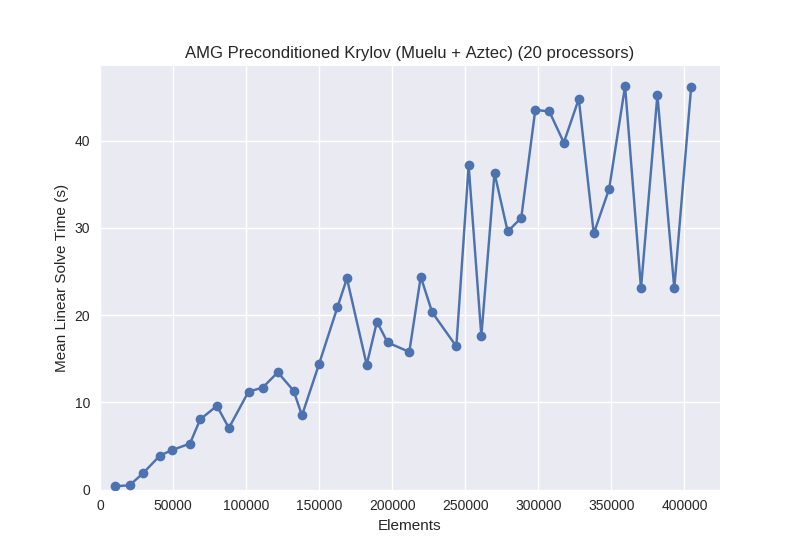
\includegraphics[width=\textwidth]{beam/muelu_beam_scaling.pdf}
%     \caption{}
% \end{subfigure}
% \begin{subfigure}{0.45\columnwidth}
%     \includegraphics[width=\textwidth]{beam/muelu_gmres_iters.pdf}
%     \caption{}
%     \label{fig:1}
% \end{subfigure}
% \end{figure}

\begin{figure}[ht]
\begin{subfigure}{\columnwidth}
    \centering
    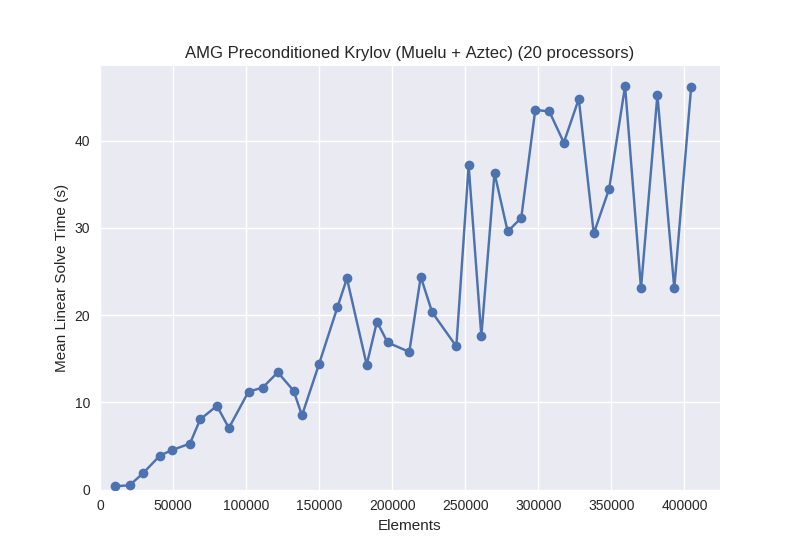
\includegraphics[width=\columnwidth]{beam/muelu_beam_scaling.pdf}
    \caption{Mean linear solve time per Newton iteration (20 Newton iterations and 10 load steps total).}
    \label{fig:weak_scaling_time}
\end{subfigure}
\begin{subfigure}{\columnwidth}
    \centering
    \includegraphics[width=\columnwidth]{beam/muelu_gmres_iters.pdf}
    \caption{Mean GMRES iterations per Newton iteration (20 Newton iterations and 10 load steps total).}
    \label{fig:weak_scaling_gmres}
\end{subfigure}
\caption{Weak scaling results (\texttildelow$10^4$ elements per core) for the cantilever beam example. Comparison of results for different beam length-to-height ratios $r$. A larger $r$-value is more slender.}
\label{fig:weak_scaling}
\end{figure}

\begin{figure}[ht]
    \begin{subfigure}{\columnwidth}
        \centering
        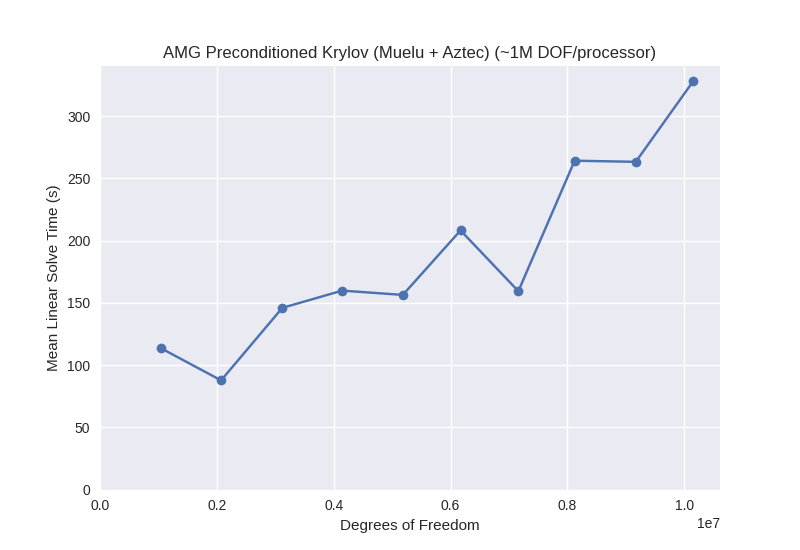
\includegraphics[width=\columnwidth]{beam_10M/muelu_ratio_10_beam_scaling.pdf}
        \caption{Mean linear solve time per Newton iteration (20 Newton iterations and 10 load steps total).}
    \end{subfigure}
    \begin{subfigure}{\columnwidth}
        \centering
        \includegraphics[width=\columnwidth]{beam_10M/muelu_ratio_10_gmres_iters.pdf}
        \caption{Mean GMRES iterations per Newton iteration (20 Newton iterations and 10 load steps total).}
    \end{subfigure}
    \caption{Weak scaling results (\texttildelow$10^6$ elements per core) for the cantilever beam example using $r = 10$.}
    \label{fig:weak_scaling_1M}
\end{figure}

\begin{figure}[ht]
    \centering
    \includegraphics[width=\columnwidth]{beam/ratio_10_prec_beam_scaling.pdf}
    \caption{Weak scaling (\texttildelow$10^4$ elements per core) solve time comparison of SuperLU direct solver against Aztec GMRES preconditioned with MueLu SA-AMG. Note that the scaling is represented on a log-scale.}
    \label{fig:superlu}
\end{figure}

\clearpage

\section{Turbojet Engine Blade}
\subsection{Problem Description}
% discussion of nullspace vectors, form for 3D elasticity
% stand-alone solver, only A was available and provided directly
For this experiment, matrices from an external finite element program were provided as the linear system to be solved. The purpose of this originally was to evaluate the feasibility of including a Krylov solver preconditioned with SA-AMG as an alternative to the sparse direct solvers already in use. The matrices as well as the right-hand side and near nullspace vectors were provided by MTU Aero Engines. The near nullspace vectors of the finest levelwere needed as separate input, so that the tentative prolongator can be calculated as in Equation~\ref{eq:prolongator_req}. For elasticity they are the rigid body modes in 3 dimensions, which for one node is

\begin{equation}
    \begin{pmatrix}
        1 & 0 & 0 & 0 & x_3 - \hat{x}_3 & \hat{x}_2 - x_2 \\
        0 & 1 & 0 & \hat{x}_3 - x_3 & 0 & x_1 - \hat{x}_1 \\
        0 & 0 & 1 & x_2 - \hat{x}_2 & \hat{x}_1 - x_1 & 0
    \end{pmatrix},
\end{equation}

where $\mathbf{x}$ is the nodal coordinate vector, $\mathbf{\hat{x}}$ is a reference point~\cite{Gee2006}. The first three columns are modes of translation in x, y, and z, respectively, and the last three columns are modes of rotation about x, y, and z, respectively. These rigid body modes can be stacked for every node in a block-wise fashion to form the necessary input for the SA-AMG preconditioner.

\subsection{Results}
The discretizations had a range of degrees of freedom from approximately 10,000 to 170,000. The original idea was to use a much larger system more representative of work done in the field. The original example contained 996,840 degrees of freedom with approximately $1.64 \cdot 10^8$ non-zero entries. Similar solver settings were used in the Muelu example, but after failure to converge, a direct solver was tried. For the direct solver, the solvers in the Amesos library were reporting detected singularities, but this was not the case with solvers used at MTU. After several attempts to diagnose the failure for the large discretization, experiments were performed with the smaller systems of the same blade. The results are shown in Figures~\ref{fig:blade1} and~\ref{fig:blade2}.

% graphs, what was tried
\begin{figure}[ht]
    \begin{subfigure}{\columnwidth}
        \centering
        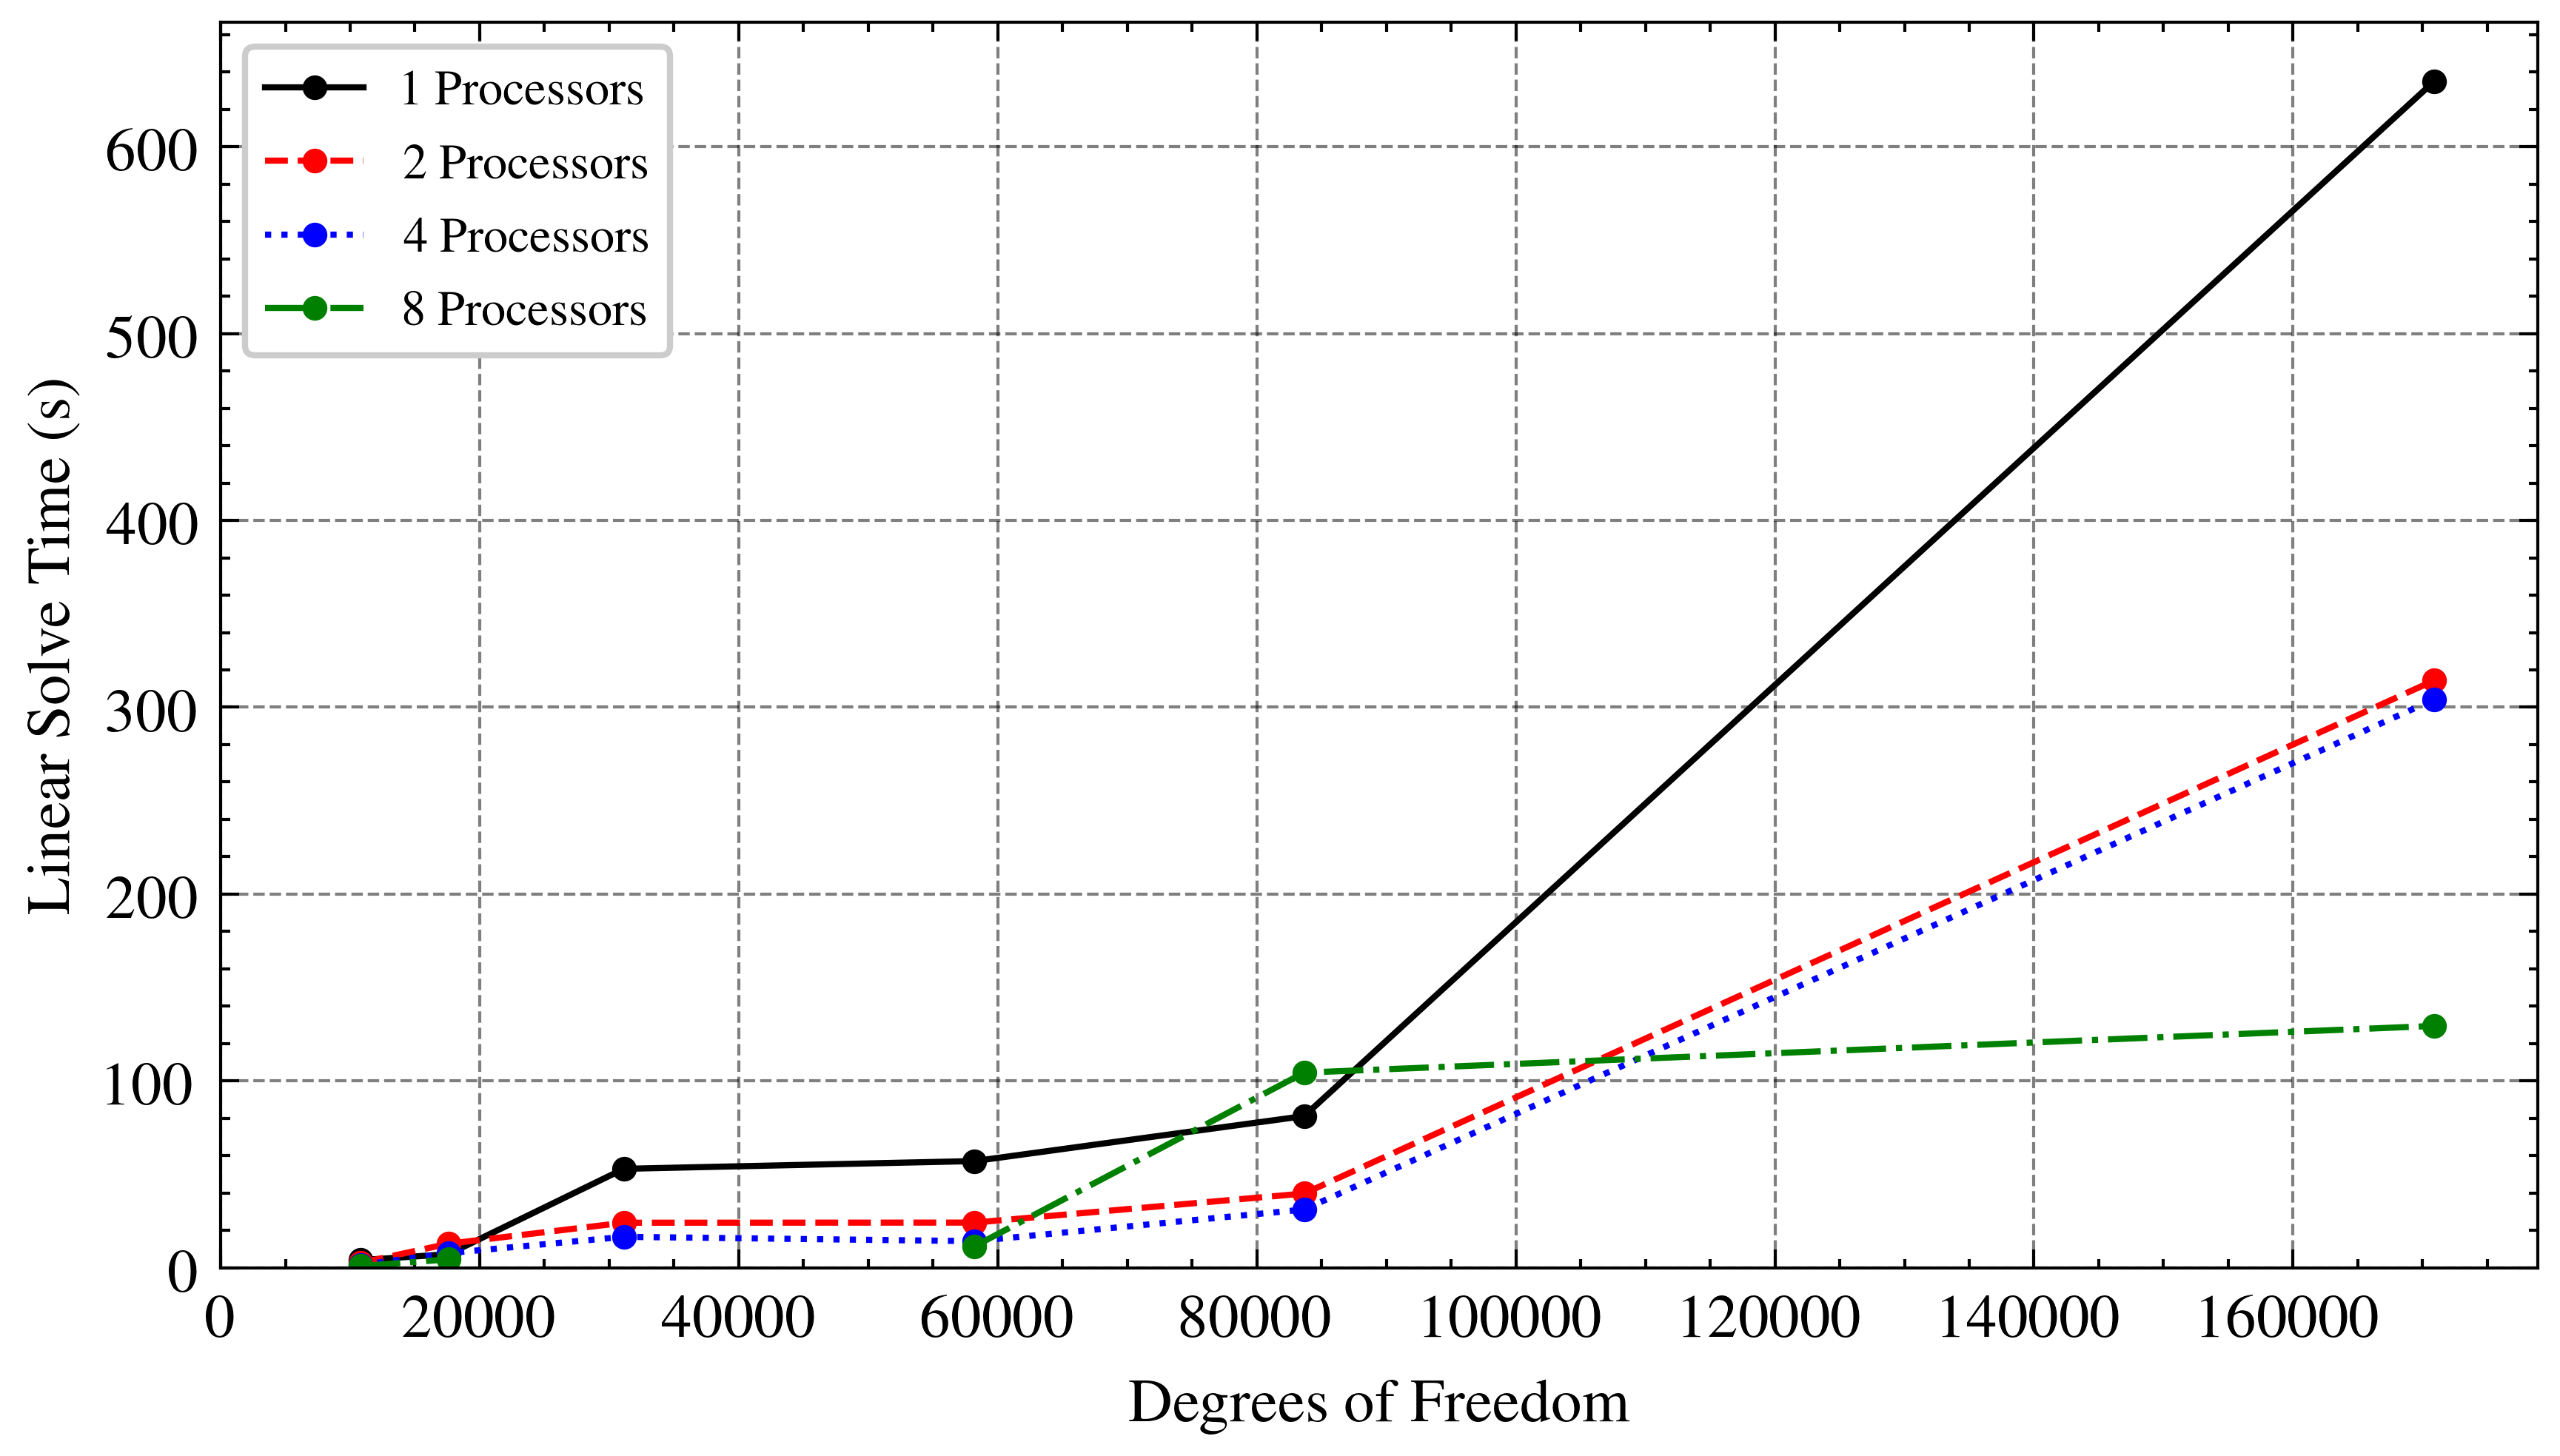
\includegraphics[width=\columnwidth]{blade/blade_klaus_small.pdf}
        \caption{Linear solve times for the various blade discretizations.}
    \end{subfigure}
    \begin{subfigure}{\columnwidth}
        \centering
        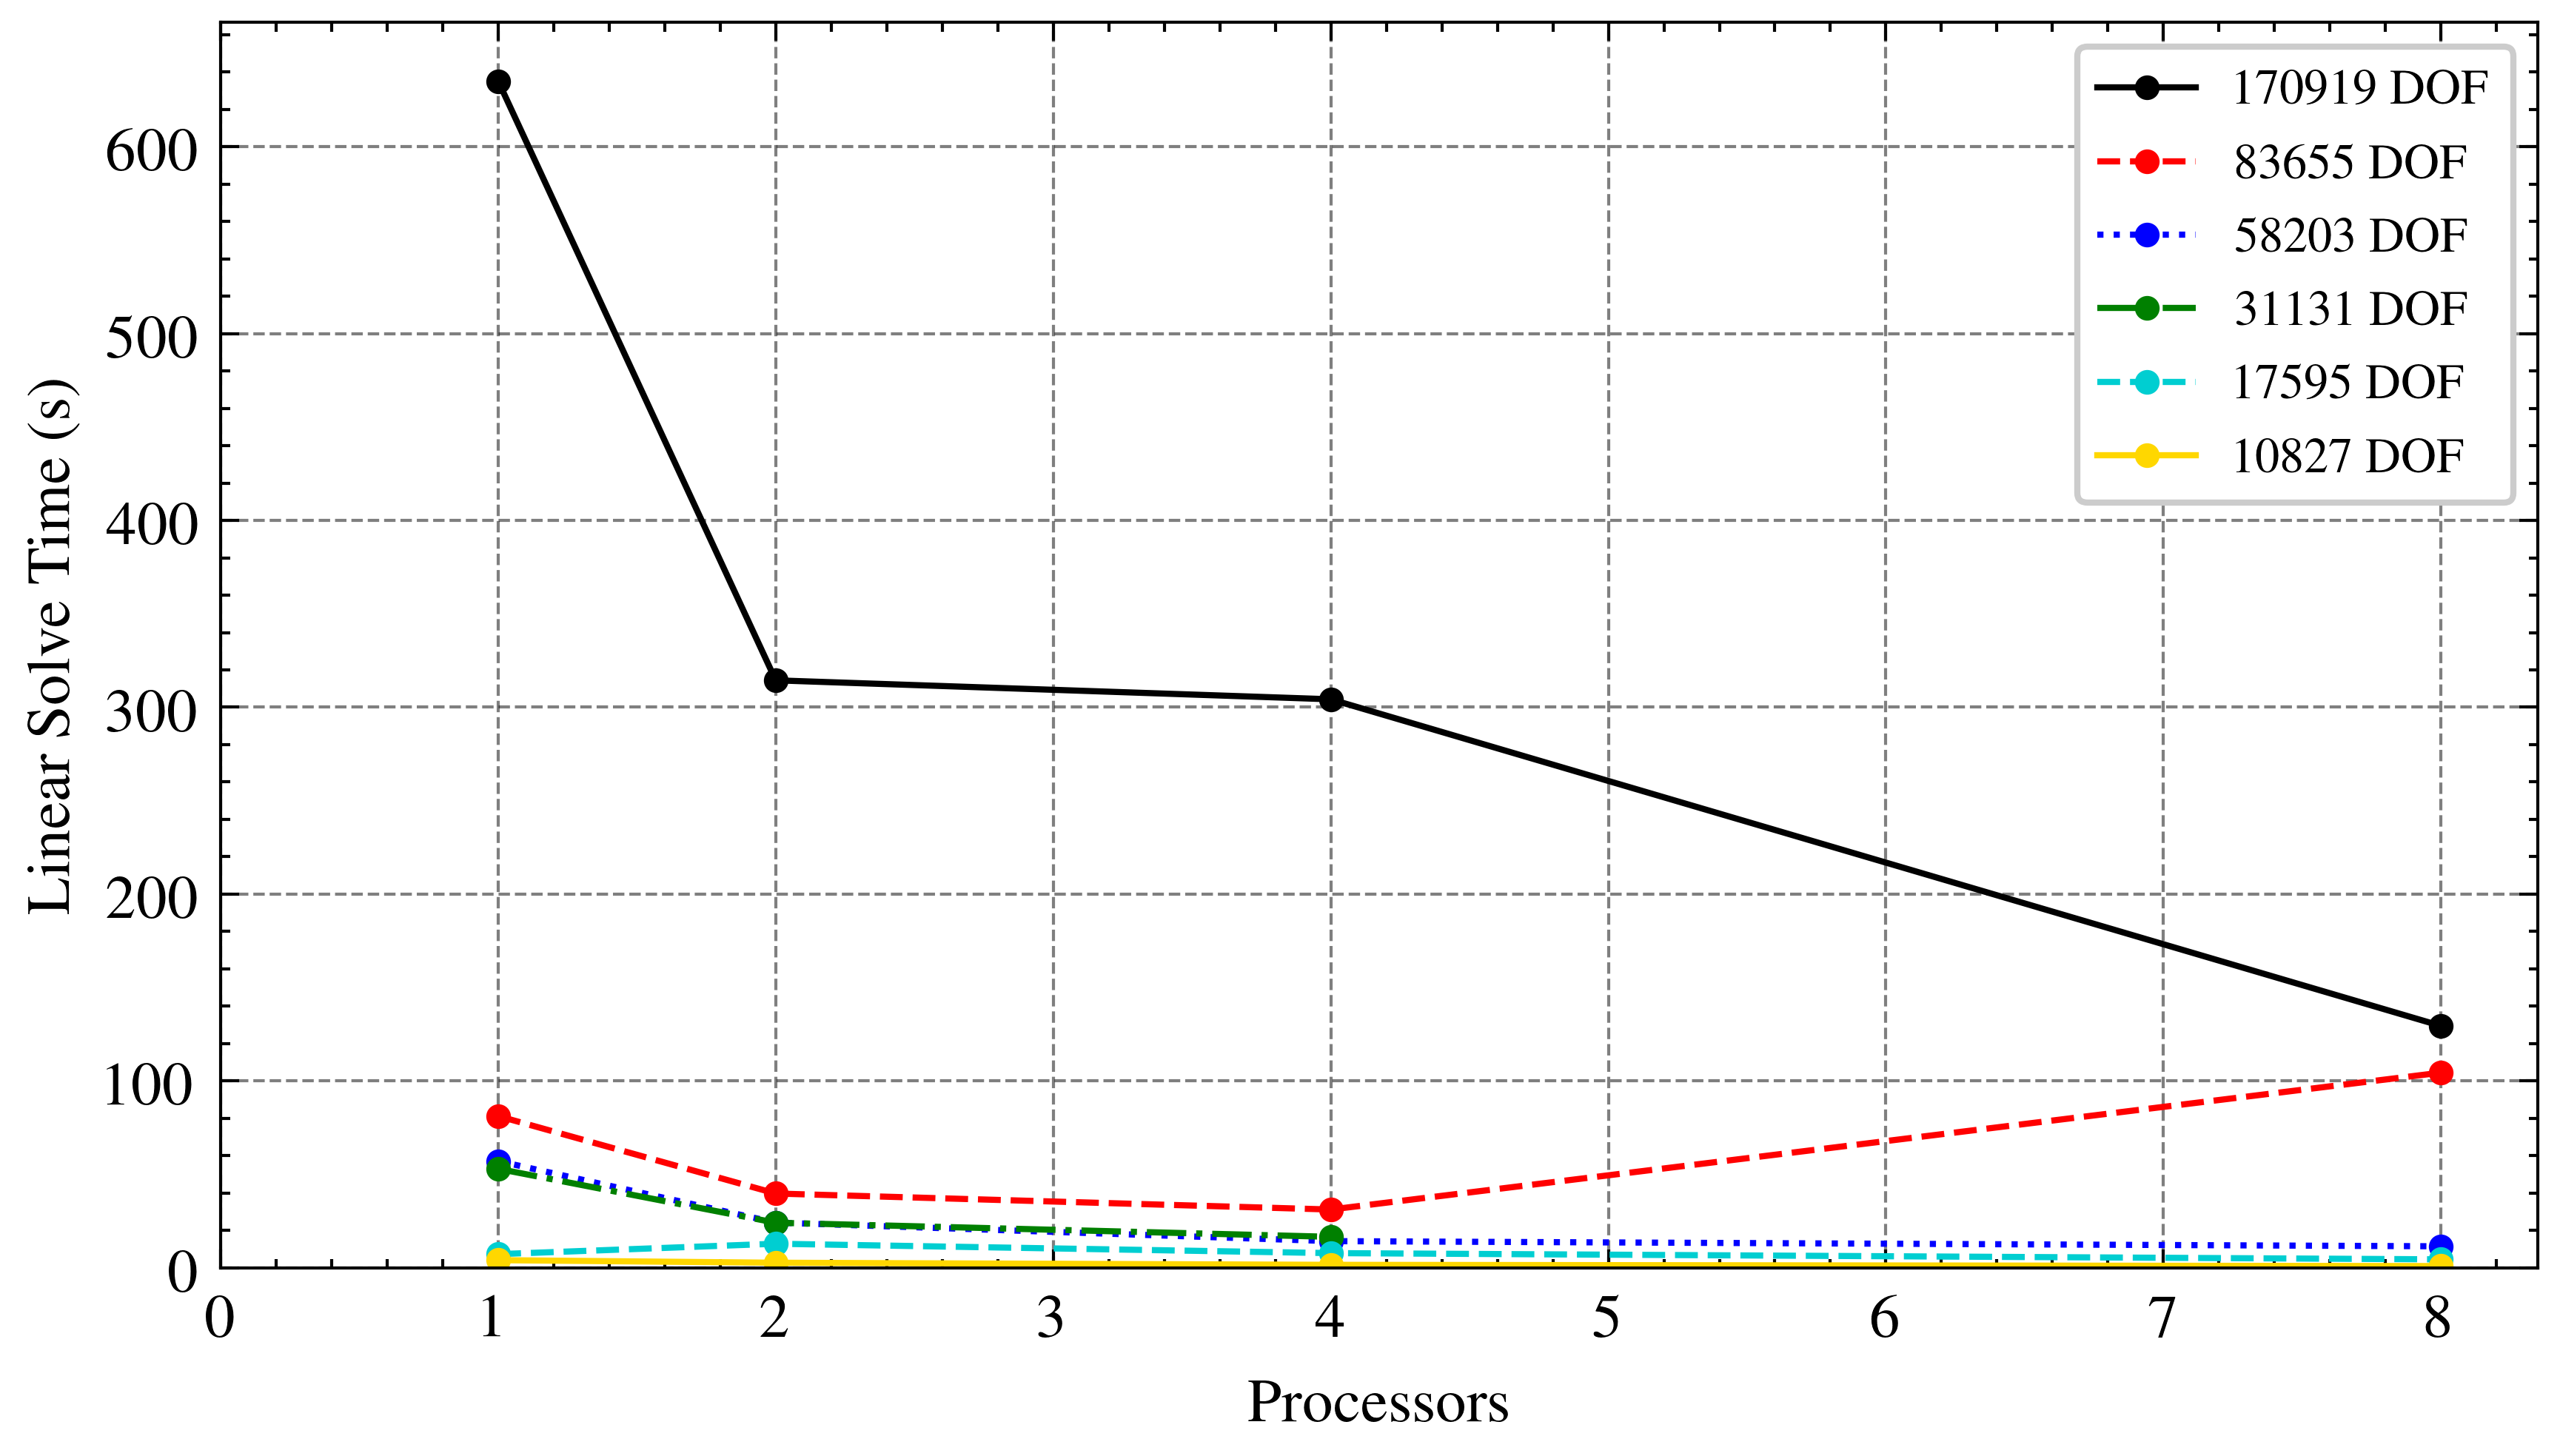
\includegraphics[width=\columnwidth]{blade/blade_klaus_small_sizes.pdf}
        \caption{Strong scaling results for the small blade discretizations.}
    \end{subfigure}
    \caption{}
    \label{fig:blade1}
\end{figure}

\begin{figure}[ht]
    \centering
    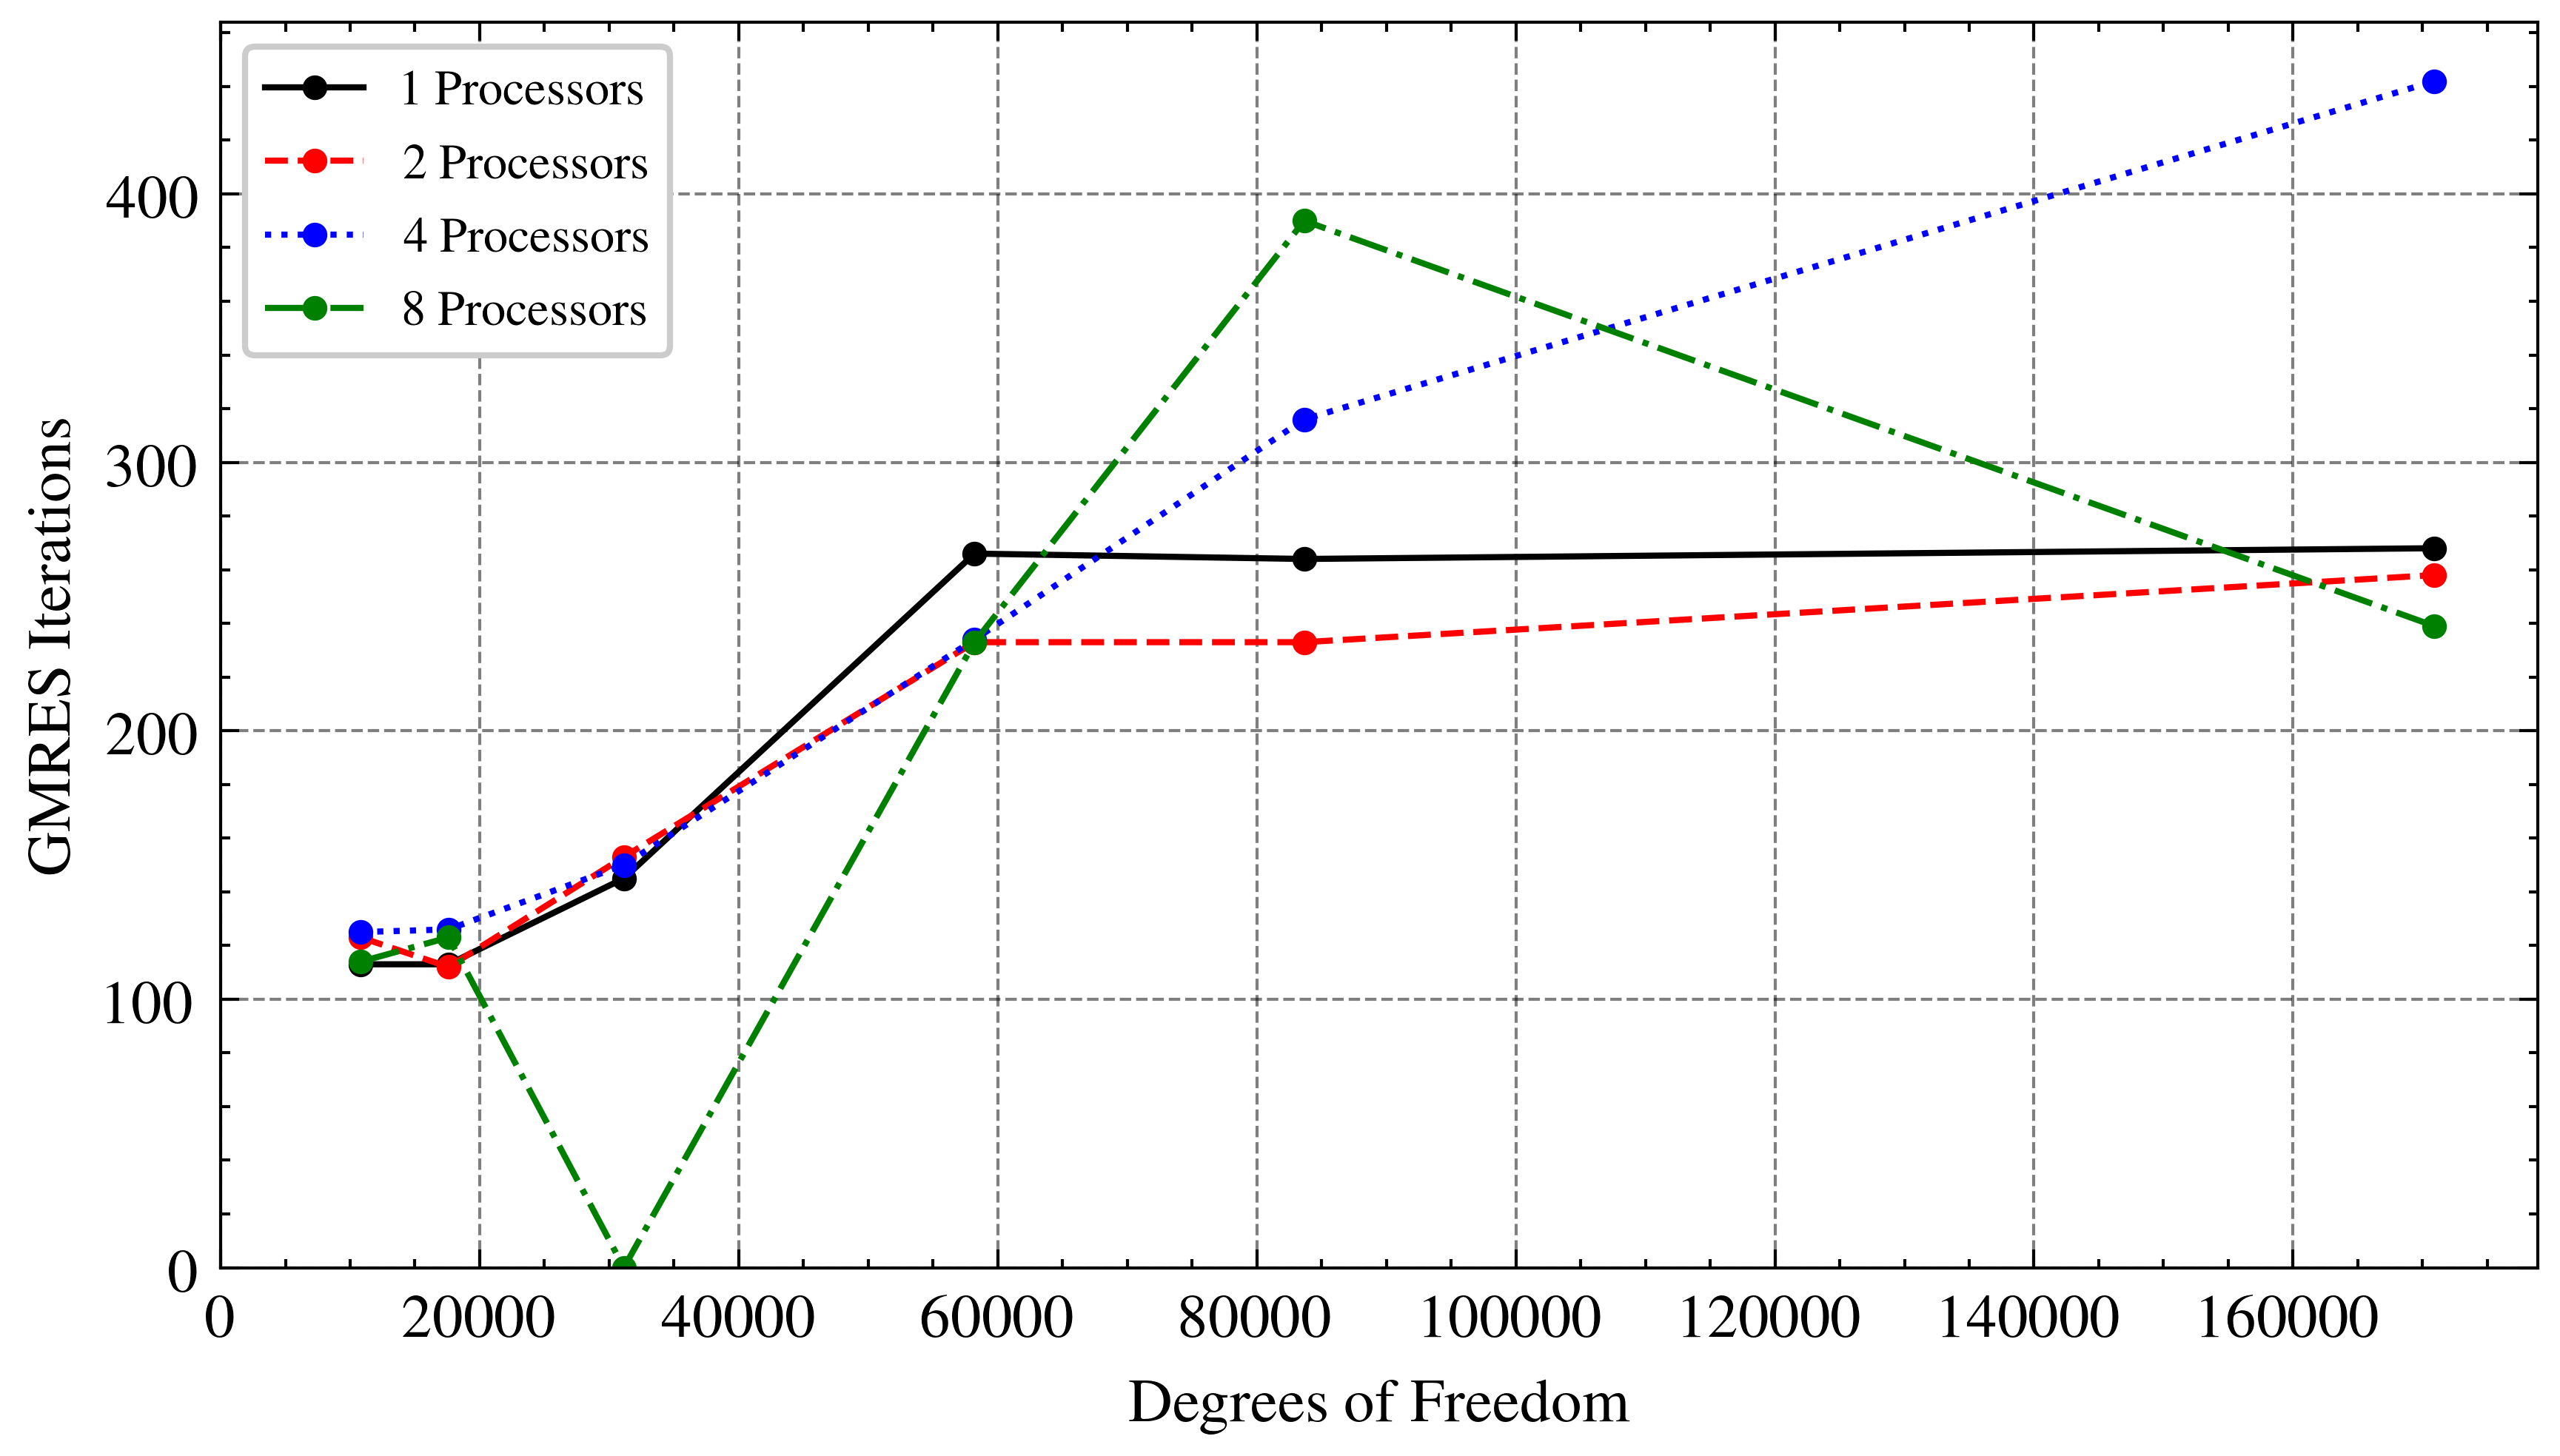
\includegraphics[width=\columnwidth]{blade/blade_klaus_small_iters.pdf}
    \caption{}
    \label{fig:blade2}
\end{figure}

\clearpage

\section{Cylindrical Shell}
\subsection{Problem Description}

\tdplotsetmaincoords{-35}{0}
\begin{figure}[ht]
  \centering
  \begin{tikzpicture}[tdplot_main_coords]
  \begin{scope}[rotate around y=-20]
    % \draw[-] (4.25,0,0) -- (4.75,0,0);
    % \draw[->] (0,0,0) -- (0,5,0) node[anchor=south]{$y$};
    % \draw[->] (0,0,0) -- (0,0,8) node[anchor=north]{$z$};
    \tdplotsetthetaplanecoords{30}
    \draw [preaction={fill=gray!40}] (4,0,0) arc[start angle=50, end angle=130, radius=4] coordinate  (b) -- ++(0,0,8.0) arc[start angle=130, end angle=50, radius=4]  -- cycle ;
    \draw [latex-latex] (4, -0.5, 8.0) arc[start angle=50, end angle=130, radius=4] node[midway, below] {$80^{\circ}$};
    \draw[latex-latex] (4.5,0,0) -- ++(0, 0, 8.0) node[midway, right] {$L = 50\ \text{cm}$};
    \node at (1.3, -0.7, 8) {$R = 25\ \text{cm}$};
    \node at (5.5, 1.7, 0) {Thickness $h = 0.25\ \text{to } 12.5$ mm};
    \draw[-] (4.25,0,0) -- (4.75,0,0);
    \draw[-] (4.25,0,8.0) -- (4.75,0,8.0);
    \draw[-] (4,0,0) arc[start angle=50, end angle=90, radius=4] -- ++(0, 1, 0) coordinate (c) --++(0, 0, 8)--++(0, -1, 0);

    \foreach \z in {0,0.5,...,8} {
        \draw[-latex] (c) +(0,0,\z) -- ++(0,-1,\z);
    }
    \node[yshift=7pt] at (c) {$\sigma_y$};
    \draw[pattern=north west lines] (4, 0, 0) --++(0.2, 0, 0) --++(0, 0, 8) --++(-0.2, 0, 0) --cycle;
    \draw[pattern=north west lines] (b) --++(-0.2, 0, 0) --++(0, 0, 8) --++(0.2, 0, 0) -- cycle;
    \node[align=left] at (7, 0, 0) {$E = 2.05 \cdot{} 10^{11}\ \text{N/m}^2$ \\ $\nu = 0.32$ \\ $\rho = 7.3 \cdot 10^3\ \text{kg/m}^3$};
  \end{scope}
\end{tikzpicture}
\caption{Cylindrical shell geometry. The straight sides are constrained with Dirichlet boundary conditions along the bottom edges, and the curved edges are free. The vertical load is applied in the middle of the shell, parallel to the straight sides.}
\end{figure}


% diagram of shell, properties used
% different height ratios, increasing force until snap through

% citing the same stuff from bischoff dissertation
% citing paper on shell stuff

\subsection{Results}

% graph/table of forces required for snap-through
%

\begin{figure}[ht]
    \centering
    \includegraphics[width=\columnwidth]{shell/shell.pdf}
    \caption{}
\end{figure}
